\chapter{Implementation}

We have implemented a system, where users can load and edits skeletons from files, or start by scratch from one skeletal node.
Our system is based on model-view-controller pattern.
Model is stored in $BMMAlgorithm$ and $BMMNode$ classes.
These classes take care of storing the skeleton, exporting skeleton to different formats and executing the base manifold mesh algorithm.
Controller is represented by $BMMController$ class.
This class prepares data from model for visualization and handles input from view.
View consists of two parts.
First, is $OpenGL$ window, which displays data provided from controller.
Second, is a Windows form, that provides Graphical User Interface (GUI) elements, which serve to make input easier.

In this chapter we will describe how we implemented our solution.
We will start with used programming language, Integrated Developer Environment (IDE), tools and libraries.
Next, we will describe implemented classes, grouped by model-view-controller pattern in greater detail.
After that we will show some programmable shaders used in our implementation.

\section{Programming Language, IDE, Tools, and Libraries}

We have selected C++ as programming language.
The main reasons are that C++ is fast and well established programming language.
Also he open source libraries that we intended to use are available for C++ and many of them are available exclusively for C++.
As IDE we are using Visual Studio 2012, which was the newest version of Visual Studio, when we started our work.
Visual Studio is supported by all of the used libraries.
We have used nVidia nSight for Visual Studio 2012 that is a debugger for graphics cards, which allows to set breakpoints in shaders during execution. We have also used several open source libraries in our project. We will briefly describe the key libraries.
To program the GPU we use OpenGL Shading Language (GLSL) version 4.3.

\begin{itemize}
	\item \textbf{Boost \cite{Boost}} Boost is a set of libraries encapsulating various task like basic input output system, smart pointers, serialization, matrices, etc. We use Boost primary for class serialization. Thanks to boost we can serialize classes into XML files, which can be stored and loaded from disk. This XML files can even be shared between different applications, so we can import skeletons from third party programs.
	\item \textbf{OpenMesh \cite{OpenMesh}} Is an open source half edge data structure library. We use it to store all meshes in our applications. OpenMesh library is capable of storing meshes composed solely from triangles as well as meshes composed of arbitrary polygons. OpenMesh has pre-calculated many convenient iterators for one-ring neighbourhoods, faces and edges adjacent to a vertex, etc. The library is also capable of exporting stored meshes into Wavefront .obj files.
	\item \textbf{GLEW \cite{glew}} The OpenGL Extension Wrangler Library (GLEW) provides efficient run-time mechanisms for activating OpenGL extensions. We use this library to expose OpenGL 4.3 functionality to our application.
	\item \textbf{OpenGL \cite{opengl}} Open source cross platform application programming interface. We use it to leverage the computation capability of GPUs to achieve hardware accelerated rendering.
	\item \textbf{GLM \cite{glm}} OpenGL Mathematics library that provides the same vector and matrix operations as available in GLSL. GLM also provides several function, that are deprecated in newer versions of OpenGL. We use this library to manipulate camera, model matrices, and for general matrix computations. GLM library is also capable of quaternion computations that are used during smoothing of BNPs and during computation of skinning matrices.
\end{itemize}

\pagebreak

\section{Classes}

Each class implements its functionality as interfaces.
These interfaces encapsulates underlying algorithms.
This allows us to replace algorithms, without affecting the rest of the code.
The relationships between the most important classes are shown in Figure \ref{fig:classes}.
Model provides interface for the controller, which allows to query models data, for visualization.
The interface provided by model also allows to change its state and attributes of various classes.
View also provides an interface for the controller, which allows the controller to display models data.
Views is also capable of receiving users input, either via mouse or by setting values exactly in an inspector panel.
Controller connects model and view together.
At constant intervals, data from model and input from view are gathered.
The model is updated according to users input and the data changes are immediately reflected in the view.

\begin{figure}[h]
    \centering
    \includegraphics[width=\textwidth]{images/classes}
    \label{fig:classes}
    \caption[Component diagram of classes]{Component diagram of most important classes, forming the model-view-controller pattern.}
\end{figure}

\subsection{Model}

Model stores the data required for our algorithm, that is the input skeleton.
Model can be in six different states, five of which mirror the steps of base mesh algorithm.
The states are: skeleton editing, skeleton straightening, BNP generation, BNP refinement, BNP joining and final vertex placement.
To input a skeleton and display the corresponding generated base mesh only skeleton editing and final vertex placement would be adequate.
However the remaining states are useful for visualization of the algorithm.
The model is designed like a library, that means it is independent from view and controller and base mesh generation can be distributed as a library.

In skeleton editing state, the input skeleton is accessible for editing.
New nodes can be added to skeletal structure.
Existing nodes can be moved, their corresponding sphere can be specified, transformation matrices can be set and leaf nodes can be set to capsules or triangle fans.
Also cyclic edges between two nodes can be specified in this state.
Outside of this state user can not edit the input skeleton by any means.

After entering skeleton straightening state the preprocessing step skeleton straightening is executed and the resulting straightened skeleton is displayed.
User can inspect the effect that skeleton straightening has on the input skeleton.

Upon entering BNP generation state the corresponding algorithm stage is executed.
User can now see polyhedrons, corresponding to each branch node, generated by spherical Delaunnay triangulation.
User can inspect faces of generated polyhedrons and display their normals.

In BNP refinement state user can see refined and smoothed polyhedrons generated by our algorithm.
The refinement procedure can be changed, after which the algorithm will be recomputed and polyhedrons smoothed with different smoothing scheme will be shown to the user.

In BNP joining state the equally named step of our algorithm is executed.
User can see straight base mesh and display normals corresponding to its faces.
It is also possible to tessellate the straightened base mesh.
The tessellation factor is global and can be adjusted from GUI.
Since the last step of the algorithm was not yet executed, elliptical nodes would appear as spherical nodes.

After entering final vertex placement state, the last step of the algorithm is executed.
User can see the final output base mesh and adjust tessellation factor.
Elliptical node have their corresponding transformations applied.
After executing any step of the base mesh algorithm user can return to any previous state, which will re-execute the algorithm again.
Application work flow is depicted in Figure \ref{fig:states}.
Direct transitions between states represent steps of the base mesh algorithm.
Transitions through junction node represent the possibility to jump between any two states in the application.

\begin{figure}[h]
    \centering
    \includegraphics[width=\textwidth]{images/states}
    \label{fig:states}
    \caption[Model state diagram]{State diagram of model. Arrows between states show application work flow. Transition between any states is possible through the junction node.}
\end{figure}

\subsubsection{BMMNode}

BMMNode is main class of the model that holds the input skeleton.
It is represented as an oriented rooted graph.
The root of the graphs is stored in BMMAlgorithm class.
The steps of base mesh algorithm are implemented in BMMNode class as recursive functions.
The functions first process the root node and then continue, with its child nodes.
All necessary data for drawing, tessellation and subsequent algorithm steps are also accessed recursively from skeletons root. All important variables are stored directly in nodes: input skeleton node position, generated polyhedron, skinning weights and other attributes required for the execution of base mesh algorithm.

\subsubsection{BMMAlgorithm}

BMMAlgorithm class provides interface that hides the underlying oriented graph and implements states discussed previously.
All queries to BMMAlgorithm are forwarded to the root node, which recursively produces output, that BMMAlgorithm returns.
This way if we would later decide to change base mesh algorithm in any way basic functionality would still be accessible through BMMALgorithm.
Furthermore BMM algorithm computes certain pre and post processing that simplifies algorithms in BMMNode.
BMMAlgorithm implements the re-rooting algorithm, so we do not need to check for invalid parents in recursive functions.
The rooted oriented graph is stored twice in BMMAlgorithm.
One copy is used to execute the base mesh algorithm itself and the other copy is used to stores the input of the algorithm, so that it can be re-executed.

\subsection{View}

View consist of Windows form components and an OpenGL view.
Windows form components are managed by Visual Studio and we are synchronizing them with our controller.
Models state is displayed in a view with OpenGL 4.3 context.
Mouse interaction in OpenGL view is recorded by our GLInput class.

\subsubsection{OpenGL view}

OpenGL view periodically queries controller for changes in model.
If model changed its state, or input skeleton was modified OpenGL view reloads buffers with new data from the model.
Otherwise view displays previously stored data.
This reduces unnecessary commands to reload buffers with data that is already stored.
Buffers are filled with data and active OpenGL programs are selected depending on models state.

In skeleton input and skeleton straightening states, buffers are filled with lines connecting skeletal nodes and spheres corresponding to each node.
Elliptical nodes transformation matrices are also stored in buffers.
Two shader programs are used to render skeletal structures.
One is specifically designed for line drawing.
The other is designed for sphere drawing.
In order to reduce the amount of data required to be send to GPU during node rendering, only one model of an icosahedron is send to GPU.
This model is then tessellated and smoothed to resemble a sphere.
Corresponding model matrices are used to position the tessellated sphere at skeleton nodes position, with appropriate scale.

BNP generation and BNP refinement states also share the same shader programs.
Upon entering these states all polyhedrons are queried from the model.
The queried polyhedrons are converted from half edge representation to indexed face representation and stored in buffers on GPU.
The shader program, responsible for rendering of polyhedrons, features one-pass wire-frame rendering and uniform shading for each triangle.
This settings are useful for visualization of generated polyhedrons.

In the last two states BNP joining and final vertex placement, the generated base mesh is converted from half edge to indexed face.
Quadrilateral parts of the mesh are send as quadrilaterals to GPU for tessellation.
Shader program for base mesh rendering displays uniformly shaded faces and wire-frame.
The shader program is also capable of Linear Blend Skinning computations, that transform the input mesh.
Currently they are used only to revert transformations applied during skeleton straightening.

\subsubsection{GLInput}

When users clicks in OpenGL view the position in view and mouse button are registered.
Mouse position is then converted from 2D view coordinates to 3D camera coordinates.
A ray with origin at mouse 3D projection and direction from camera to mouse 3D projection is casted in the scene.
The process is shown in Figure \ref{fig:camera_selection}.
The mouse 2D location was mapped onto near plane and yellow ray was casted into the scene.
The first hit object is then selected.
Mouse actions are context dependant.

If the ray intersects a node the node is selected, its corresponding attributes are displayed in the inspector.
A selected node can be moved in the scene and this way its position attributes are updated.
With selected node user can create new nodes as child of selected node with middle click of the mouse.
Right clicking on a different node creates a cycle between selected and clicked node.
User can also rotated child nodes of a node.
In this mode left, right and middle clicks produce rotations around X, Y and Z axis respectively.

If after tracing the ray we do not encounter a node the resulting interaction is handled as rotations and translations of camera.
Camera is locked on a point and can be rotated around that point by right clicking in the scene.
A left click moves the point in a plane that is parallel to near plane of the camera.
Mouse wheel translates the camera along its view direction and therefore produces the effect of zooming in and out with the camera.

\begin{figure}[h]
    \centering
    \includegraphics[width=\textwidth]{images/camera_selection}
    \label{fig:camera_selection}
    \caption[Camera selection]{Camera selection in 3D. Mouse 2D location is mapped onto near plane and a ray is casted through the scene. The first object hit by the ray is selected.}
\end{figure}

\subsection{Controller}

Controller updates input forms with models data and if new values are provided through input forms controller updates model accordingly.

\section{GPU Shaders}